\subsection{Paraboloids}
\noindent
The paraboloid looks like a parabola that has been rotated and extruded about its axis of symmetry.
It is radially symmetric, and its level curves are circles.
Paraboloids have the form $z = ax^2 + by^2$ where $a,b \in \mathbb{R}$.

\begin{figure}[H]
	\centering
	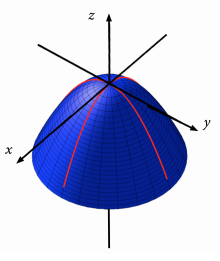
\includegraphics[width = 0.3\textwidth]{./differentialMultivariableCalculus/paraboloid.png}
	\caption{A paraboloid}
\end{figure}